% =============================================================================
% N1-LoSt: paper template
%
% Location: <repo>/paper/main.tex
% Figures:  read from <repo>/Output/ (see \outdir below)
% Build:    latexmk -pdf main.tex   (or "Build LaTeX project" in VS Code)
% =============================================================================
\documentclass[11pt,a4paper]{article}

% --- Encoding, fonts, layout -------------------------------------------------
\usepackage[utf8]{inputenc}
\usepackage[T1]{fontenc}
\usepackage{lmodern}  % scalable fonts (needed by microtype)
\usepackage{microtype}
\usepackage[margin=2.5cm]{geometry}
\usepackage{setspace}
\onehalfspacing

% --- Maths, units, tables ----------------------------------------------------
\usepackage{amsmath,amssymb}
\usepackage{siunitx}
\usepackage{booktabs}
\usepackage{tabularx}

% --- Figures -----------------------------------------------------------------
\usepackage{graphicx}
\usepackage{caption}
\usepackage{subcaption}
\usepackage{float}

% --- Authors and affiliations ------------------------------------------------
\usepackage{authblk}

% --- Line numbers (useful for drafts and reviews; comment out for final) ----
\usepackage{lineno}
\linenumbers

% --- References --------------------------------------------------------------
\usepackage[numbers,sort&compress]{natbib}
\bibliographystyle{unsrtnat}

% --- Links (load last) -------------------------------------------------------
\usepackage[hidelinks]{hyperref}

% =============================================================================
% Figures from the Output folder of the repository
% =============================================================================
\newcommand{\outdir}{../Output/}

% \outfig{path inside Output}{width as fraction of \textwidth}{caption}{label}
% If the file does not exist, a box with its path is shown instead.
\newcommand{\outfig}[4]{%
  \begin{figure}[htbp]
    \centering
    \IfFileExists{\outdir#1}%
      {\includegraphics[width=#2\textwidth]{\outdir#1}}%
      {\fbox{\parbox[c][4cm][c]{0.8\textwidth}{\centering\small Missing figure:\\
        \texttt{\detokenize{#1}}}}}%
    \caption{#3}\label{#4}
  \end{figure}}

% Same, without the figure environment (for subfigures)
\newcommand{\outimg}[2]{%
  \IfFileExists{\outdir#1}%
    {\includegraphics[width=#2\linewidth]{\outdir#1}}%
    {\fbox{\parbox[c][3cm][c]{0.9\linewidth}{\centering\scriptsize Missing:\\
      \texttt{\detokenize{#1}}}}}}

% =============================================================================
% Title
% =============================================================================
\title{N-of-1 Longitudinal Study of a Patient with ME/CFS: Methods and Preliminary Results}
\author[1]{Paolo Maccallini}
\affil[1]{``Independent researcher'', Rome, Italy}
\date{\today}

\begin{document}
\maketitle

% =============================================================================
\begin{abstract}
% Background, methods, results, conclusions (about 250 words).

\end{abstract}

\noindent\textbf{Keywords:} n-of-1; intensive longitudinal data; ME/CFS; fNIRS; EEG; 
HRV; POTS

% =============================================================================
\section{Introduction}\label{sec:introduction}
% =============================================================================


% =============================================================================
\section{Methods}\label{sec:methods}
% =============================================================================

\subsection{Study design}\label{sec:design}


\subsection{Data acquisition}\label{sec:acquisition}

\subsubsection{Symptom scores}

\subsubsection{Physical activity}

Daily step counts were recorded with a smartphone (Redmi Note 11S/Pedometer Step Counter) 
from January 2023, and with a wrist-worn watch (Dyurawa) from March 2025. The phone records only the
steps taken while it is carried, so it misses most activity at home, whereas the watch
records activity throughout the day; watch counts were therefore taken as the reference
measure.

Gaps of up to four consecutive days were filled by linear interpolation in both series, if missing
days were less than 10\%. Days on which the watch recorded fewer steps than the phone were considered days of
watch non-wear or malfunction, and their watch counts were set to missing.

To obtain a continuous series of watch-equivalent steps over the whole study period
(\texttt{Steps.C}), watch counts were estimated from phone counts on days without watch
data. The relationship between the two counts differs between days spent at home, when
the phone is mostly not carried and its count carries little information, and days with
outdoor activity, when the phone is carried. Days were therefore divided into two regimes
by a threshold $t$ on phone steps (\texttt{Steps}), and a linear regression of watch steps 
(\texttt{Steps.B}) on phone steps was fitted separately in each regime. The threshold was chosen by scanning values from
50 to 2000 phone steps and selecting the one that minimised the total sum of squared
residuals of the two regressions, requiring at least 20 days in each regime
(see Figure~\ref{fig:steps-model}). On days with watch data,
\texttt{Steps.C} equals the measured watch count; on the other days, it is the value
predicted by the regression of the corresponding regime.

The imputation was validated by fitting the model on the first 80\% of the watch period
and comparing the values predicted for the remaining 20\% with the measured ones (Figure~\ref{fig:steps-validation}). 
The relative mean absolute error, $\sum|\hat{y}_i - y_i| / \sum y_i$, and the relative mean error
(bias), $\sum(\hat{y}_i - y_i) / \sum y_i$, are indicated on the plot. Most days were slightly overestimated,
while the most active days, and outdoor activity without the phone, were underestimated. The time series 
of \texttt{Steps}, \texttt{Steps.B}, and \texttt{Steps.C} are shown in Figure~\ref{fig:steps}.

\begin{figure}[htbp]
  \centering
  \begin{subfigure}{0.48\textwidth}
    \centering
    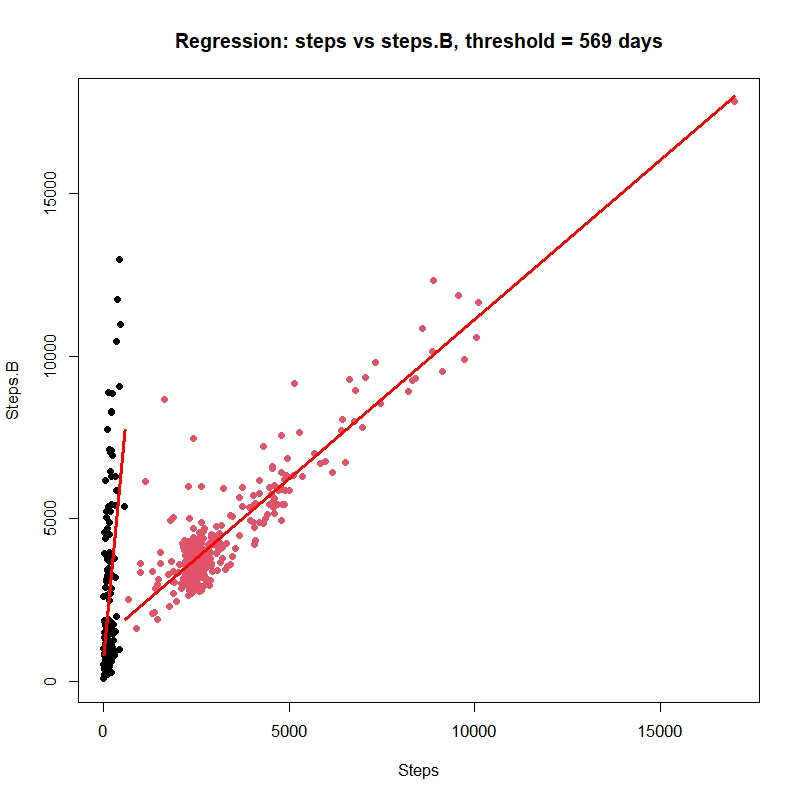
\includegraphics[width=\linewidth]{../Output/Steps/regression_model.jpg}
    \caption{Regression model.}\label{fig:steps-model}
  \end{subfigure}\hfill
  \begin{subfigure}{0.48\textwidth}
    \centering
    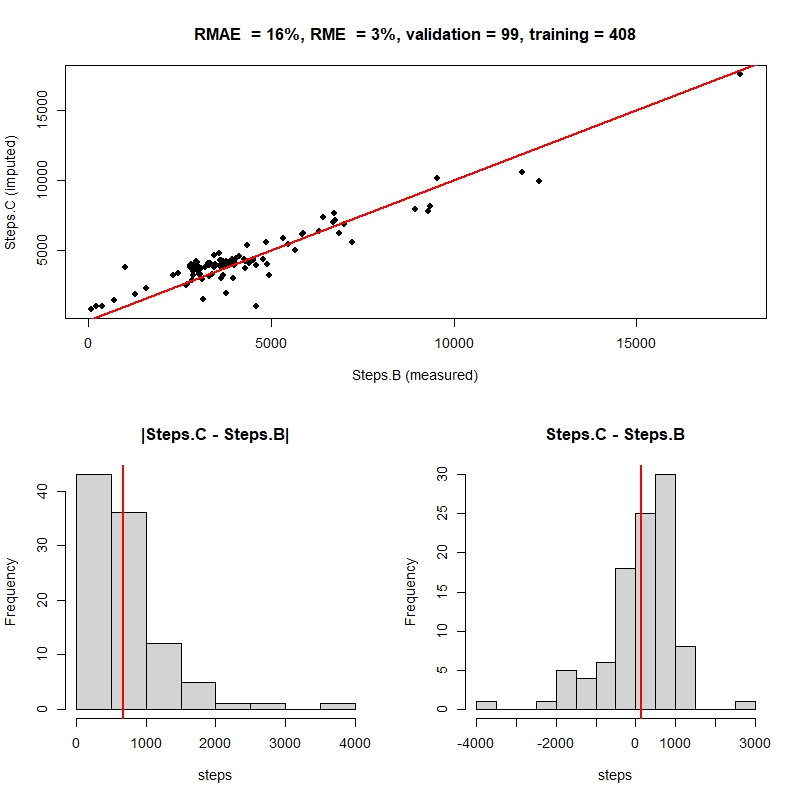
\includegraphics[width=\linewidth]{../Output/Steps/regression_validation.jpg}
    \caption{Validation.}\label{fig:steps-validation}
  \end{subfigure}
  \caption{Imputation of watch steps (\texttt{Steps.B}) from phone steps (\texttt{Steps}).}\label{fig:steps}
\end{figure}

\begin{figure}[htbp]
  \centering
  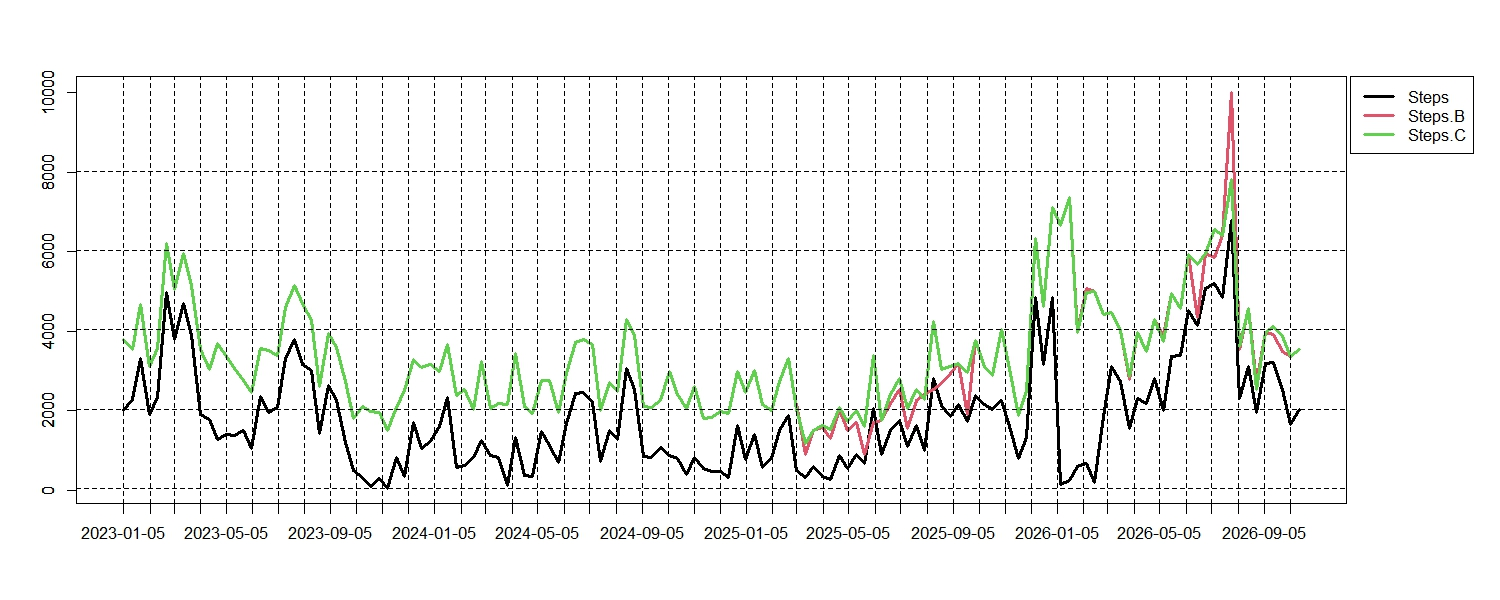
\includegraphics[width=\textwidth]{../Output/Steps/normplot_10_Steps.jpeg}
  \caption{Daily steps averaged over non-overlapping 10-day blocks.}
  \label{fig:steps}
\end{figure}

\subsubsection{Heart rate variability}

\subsubsection{Blood pressure and lean test}

\subsubsection{Body composition}

\subsubsection{Indoor and outdoor environment}

\subsubsection{EEG and fNIRS}

\subsubsection{Blood tests}

\subsubsection{Drugs and supplements}


\subsection{Data processing}\label{sec:processing}


\subsection{Statistical analysis}\label{sec:statistics}


% =============================================================================
\section{Results}\label{sec:results}
% =============================================================================

% Example: single figure from Output/
\outfig{Time_series/fourier.jpeg}{0.8}
  {CAPTION.}
  {fig:fourier}

% Example: two figures side by side
\begin{figure}[htbp]
  \centering
  \begin{subfigure}{0.48\textwidth}
    \centering
    \outimg{Time_series/decomposition.jpeg}{1}
    \caption{CAPTION A.}\label{fig:pair-a}
  \end{subfigure}\hfill
  \begin{subfigure}{0.48\textwidth}
    \centering
    \outimg{steps.jpg}{1}
    \caption{CAPTION B.}\label{fig:pair-b}
  \end{subfigure}
  \caption{CAPTION OF THE PAIR.}\label{fig:pair}
\end{figure}

% Example: table
\begin{table}[htbp]
  \centering
  \caption{CAPTION.}\label{tab:example}
  \begin{tabular}{lrr}
    \toprule
    Variable & Value & Unit \\
    \midrule
    NAME & 0.0 & \si{ms} \\
    \bottomrule
  \end{tabular}
\end{table}

% Example of references in the text:
% as shown in Figure~\ref{fig:fourier} and Table~\ref{tab:example} \citep{bh1995}.


% =============================================================================
\section{Discussion}\label{sec:discussion}
% =============================================================================

\subsection{Limitations}\label{sec:limitations}


% =============================================================================
\section{Conclusions}\label{sec:conclusions}
% =============================================================================


% =============================================================================
\section*{Data and code availability}
% =============================================================================
Code: \url{https://github.com/USERNAME/N1-LoSt}.


% =============================================================================
\section*{Acknowledgements}
% =============================================================================


% =============================================================================
\bibliography{refs}

% =============================================================================
\appendix
\section{Supplementary material}\label{sec:appendix}
% =============================================================================


\end{document}
